%% LyX 2.2.0 created this file.  For more info, see http://www.lyx.org/.
%% Do not edit unless you really know what you are doing.
\documentclass[12pt,english]{kuthesis}
\usepackage{mathptmx}
\usepackage{amssymb}
\renewcommand{\sfdefault}{lmss}
\renewcommand{\ttdefault}{lmtt}
\usepackage[T1]{fontenc}
\usepackage[utf8]{inputenc}
\usepackage{geometry}
\geometry{verbose,tmargin=1in,bmargin=1in,lmargin=1in,rmargin=1in}
\setcounter{secnumdepth}{3}
\setcounter{tocdepth}{3}
\usepackage{color}
\usepackage{babel}
\usepackage{url}
\usepackage{graphicx}
\usepackage{setspace}
\usepackage{esint}
\usepackage[authoryear]{natbib}
\doublespacing
\usepackage[unicode=true,
 bookmarks=true,bookmarksnumbered=false,bookmarksopen=false,
 breaklinks=true,pdfborder={0 0 0},pdfborderstyle={},backref=false,colorlinks=true]
 {hyperref}
\hypersetup{pdftitle={University of Kansas Thesis Template},
 pdfauthor={Anonymous},
 pdfsubject={A Thesis},
 urlcolor={black},citecolor={black},allcolors={black}}

\makeatletter

%%%%%%%%%%%%%%%%%%%%%%%%%%%%%% LyX specific LaTeX commands.
\providecommand{\LyX}{\texorpdfstring%
  {L\kern-.1667em\lower.25em\hbox{Y}\kern-.125emX\@}
  {LyX}}
%% Because html converters don't know tabularnewline
\providecommand{\tabularnewline}{\\}

%%%%%%%%%%%%%%%%%%%%%%%%%%%%%% User specified LaTeX commands.


%used to align decimals in tables according to APA style
\usepackage{dcolumn}
\usepackage{booktabs}

% Set the title and author info
\title{Please Read the Abstract}
\author{Abstract Writer}


\dept{Department of People who read Abstracts}
\degreetitle{Doctor of Philosophy}
\papertype{Thesis} %or Thesis (Whatever you put will appear on p.2)
%% It is vital to have 7 entries, even if some are empty for committee and role
%% I mean, it is vital to leave the empty place holders
\committee{MEMBER 1}{MEMBER 2}{MEMBER 3}{MEMBER 4}{The One with an Extra Long Name}{The Fifth Beatle}{}
\role{Chairperson}{Occasional Visitor}{}{The One Who Never Answers Email}{}{}{}
%AT Most 7 members allowed, last here is blank on purpose to demonstrate
%flexibility

%% The following is OPTIONAL. Remove all 3 of the next 3 lines
%% to leave dates blank. If dates are included, then both dates 
%% must be included.
\@printd@testrue
\datedefended{October 02, 2016}
\dateapproved{October 06, 2016}

%% These settings are now in the kuthesis.cls file, but users are free
% to customize. listings has great documentation online
%% When listings are used, break lines
%\lstset{
 %    breaklines=true,  % sets automatic line breaking
 %    breakindent=2em,
 %    breakatwhitespace=true,  % sets if automatic breaks should
 %   breakautoindent=true
%}

\@ifundefined{showcaptionsetup}{}{%
 \PassOptionsToPackage{caption=false}{subfig}}
\usepackage{subfig}
\makeatother

\usepackage{listings}
\renewcommand{\lstlistingname}{\inputencoding{latin9}Listing}

\begin{document}
\begin{romanpages}

\maketitle
\begin{abstract}

%The diffractive dijet photoproduction can probe the nuclear parton distribution at low Bjorken-x.

\begin{acknowledgementslong}

%%if you want a "quote" environment for acknowledgements,
%% use acknowledgements instead of acknowledgementslong

%Thanks to my family and friends.

\end{acknowledgementslong}
\end{abstract}
\tableofcontents{}

\listoffigures
\listoftables

\end{romanpages}

\setlength\abovedisplayskip{0pt}

\chapter{Ultra-relativistic heavy-ion collisions}

\section{The Standard Model}

The Standard Model describes the fundamental particles of the universe in terms of fermions and bosons. Fermions are particles with half-integer spin, while bosons have integer-spin. This difference in spin has far reaching consequences. Fermions must obey the Pauli Exclusion Principle: only one fermion at a time can occupy a given state. However, multiple bosons can simultaneously occupy a specific state. Subnuclear particles -- protons and neutrons -- contain large numbers of both fermions and bosons. 

Among the fermions are the leptons, neutrinos, and quarks. The leptons consist of the electron, muon, and tau, as well as their anti-particles. The leptons are seemingly fundamental: high energy experiments have yet to observe internal lepton-structure. Neutrinos are weakly interacting particles detected primarily through the precise measuring of missing transverse energy in the products of particle collisions. Quarks are the constituent particles of baryons, which contain three valence quarks, and mesons, which contain two valence quarks. In addition to the valence quarks are the sea quarks, which appear and disappear as quark-antiquark pairs within hadrons. The hadrons are particles made of quarks and gluons. Gluons are particles that mediate the strong nuclear force; likewise, photons mediate the electromagnetic force, and weak-gauge bosons mediate the weak nuclear force. A fourth boson, the graviton, is expected to transmit the gravitational force, but this particles existence has not been verified. 

The behavior of fundamental particles is best described within the framework of quantum field theory (QTF). QFT defines a Lagrangian for fundamental particles. This Lagrangian then predicts the outcome of particle collisions. Different terms in the Lagrangian correspond to the various interactions between particles. The Standard Model Lagrangian, $\mathcal{L}_{Standard Model}$ can be broken down into three basic terms:	
\begin{equation}
\mathcal{L}_{Standard Model} = \mathcal{L}_{QED} + \mathcal{L}_{QCD} + \mathcal{L}_{Higgs} + ... ,  
\end{equation}
Where $\mathcal{L}_{QED}$ is the QED Lagrangin, $\mathcal{L}_{QCD}$ is the QCD Lagrangian, and $\mathcal{L}_{Higgs}$ is the Higgs Lagrangian. The QED and QCD Lagrangians will be the most important in what follows \cite{Halzen:1984mc}. 

The most accessible approach to quantum field theory is through the use of Feynman diagrams. First, one imagines an interaction between particles. Then, one draws this process into a Feynman diagram, which is essentially a pictorial representation of exchanges between particles. The Lagrangian can be interpreted into Feynman rules. These rules describe how the Feynman diagram translates into a calcuation for the quantum mechanical amplitude of the process. The quantum mechanical amplitude, in turn, is proportional to the cross-section of the process. This is important because, sense the cross-section is invariant between experiments, one can use it to effectively test for invariant quantities in the Lagrangian \cite{Peskin:1995ev}.

\section{Quantum electrodynamics}

In classical electrodynamics, all of electrical and magnetic phenomena can be derived from four fundamental equations: Maxwell's laws. Below these equations are given in their differential form. 

Gauss's law relates the divergence of a static electric field, $\vec{E}$, to it's source charge density, $\rho$,
\begin{equation}
\triangledown\cdot\vec{E}= \frac{\rho}{\epsilon_o},
\end{equation}
where $\epsilon_o$ is permittivity of free space. Gauss's law for a static magnetic field, $\vec{B}$, reveals the stark contrast between electricity and magnetism. The diverence of a static magnetic field is always a net 0. This reflects the seeming non-existence of magnetic monopoles.  
\begin{equation}
\triangledown\cdot\vec{B}=0
\end{equation}
Faraday's law describes the curl of an electric field in terms of the dynamics of a magnetic field. The electric field and the magnetic field are coupled, and a change in one will affect the properties of the other. For a given electric field, $\vec{E}$, the curl is equal to the partial derivative of a magnetic field, $\vec{B}$, with respect to time, $t$,
\begin{equation}
\triangledown\times\vec{E}=-\frac{\partial\vec{B}}{\partial t}.
\end{equation}
Ampere's law addresses the curl of a magnetic field, $\vec{B}$, and once more the absence of magnetic monopoles gives rise to distinct properties. In addition to the partial derivative of $\vec{E}$ with respect to time $t$, there is a corrective term for the electric charge current density, $\vec{J}$, and the sum is multiplied by $\mu_o$, the permeability of free space,
\begin{equation}
\triangledown \times \vec{B} = \mu_o \left(  \vec{J} + \epsilon _{o} \frac{\partial \vec{E}}{\partial t} \right ).
\end{equation}
The complementarity of the classical electric and magnetic fields gives rise to the photon flux so important for ultra-peripheral collisions, and will be discussed in greater detail in the next chapter.

\begin{equation}
{\mathcal {L}}={\bar {\psi }}(i\gamma ^{\mu }D_{\mu }-m)\psi -{\frac {1}{4}}F_{\mu \nu }F^{\mu \nu }
\end{equation} 

Quantum electrodynamics (QED) is a theory of electromagnetic interaction in terms of relativistic quantum field theory. QED addresses three specific processes: photon motion, electron motion, and the emission, or absorption, of a photon by an electron. To do this, first a Lagrangian is established based on Maxwell's laws and quantum mechanics. The photon constitutes a spin-1 solution to Maxwell's equations. Likewise, electrons are described, at non-relativistic scales, by the Schrodinger equation, at relativistic scales by the Dirac equation. Figure \ref{fig:qedFeynman} shows the resulting processes allowed by QED: the translation of an electron, the translation of a photon, and the scattering of a photon off an electron \cite{Griffiths:2008zz}.

\begin{figure}[h!]
\begin{centering}
\includegraphics[width=4in]{Chapter1/importfigs/Feynman_Diagram_Components.png}
\par\end{centering}
\caption{QED Components of Feynman Diagrams (Plot from WikiCommons). \label{fig:qedFeynman}}
\end{figure}

The QED coupling constant, $\alpha_QED$, is approximately ~1/137 at perturbative scales. However, at small scales, i.e. non-perturbative momentum transfers $Q^2$, the coupling constant increases:
\begin{equation}
\alpha_{QED}(Q^2) = \frac{ \alpha_{em}}{(1 - \frac{\alpha_{em}}{3\pi})\mathrm{ln}(\frac{Q^2}{m^2}) },
\end{equation}
where $\alpha_{QED}(Q^2)$ is the QED coupling constant at high $Q^2$, $\alpha_{em}$, and $m$ is the electron mass. High values of $Q^2$ are non-perturbative because, at small scales and high momentum, the fluctuation of photons into electron-positron pairs begins to saturate.

\section{Quantum chromodynamics}

The quarks are a family of fermions that compose the baryons and the mesons. Baryons consist of three quarks in a color neutral state, while mesons consist two quarks in a color neutral state. "Color" in this context refers to the six kinds of strongly-interacting charge available to quarks: red and anti-red, blue and anti-blue, and green and anti-green. Color charge has no relation to optical phenomena, but provides a useful analogy for the stable combinations of quarks. The net color-charge of a baryon or meson is colorless. By way of analogy, a red quark, green quark, and blue quark can together form a hadron, in the way that conventional red, green, and blue can together form white \cite{Brock:1993sz}. 

Gluons are the QCD analogues of the photons in QED. Gluons are spin-1 and massless, but unlike photons, which do not carry electromagnetic charge, gluons carry strongly-interacting charge: color. Color comes six varieties: red, antired, blue, antiblue, green, and antigreen \cite{Wilczek:2000ih}. 

Unlike QED, the QCD coupling increases with distance \cite{Bethke:2006ac}. Figure \ref{fig:runningQCDCoupling} shows the running of the QCD coupling with $Q^2$:
\begin{equation}
\alpha_{QCD}(Q^2) = \frac{4 \pi }{(11 - \frac{2}{3}n_f)\mathrm{ln}(\frac{Q^2}{\Lambda^2_{QCD}}) } ,
\end{equation}
where $n_f$ is the number of quark flavors, $Q^2$ is the momentum transfer, and  $\Lambda^2_{QCD}$ is the mass scale. 
This has the practical consequence of the strong-interactions being stronger in high momentum transfer collisions. The direct results of the running QCD coupling are the dual phenomena of asymptotic freedom and color confinement. At large distances, string tension describes the binding force of the quarks. At short distances, however, Coulomb-like interactions dominate. The QCD coupling constant can be measured via the cross-section of inelastic proton-proton collisions, and also the cross section of electron-positrons into triple jets. 
\begin{figure}[h!]
\begin{centering}
\includegraphics[width=4in]{Chapter1/importfigs/qcd_coupling_bethke.png}
\par\end{centering}
\caption{QCD Coupling Constant vs. $Q^2$ \cite{Bethke:2006ac} \label{fig:runningQCDCoupling}}
\end{figure}

Within the nucleus, a proton can be thought of as a bubble in a vacuum. Debrye screening exerts a pressure on the proton. This pressure is responsible for the size of the proton. 

\begin{equation}
{\mathcal {L}}_{\mathrm {QCD} }={\bar {\psi }}_{i}\left(i(\gamma ^{\mu }D_{\mu })_{ij}-m\,\delta _{ij}\right)\psi _{j}-{\frac {1}{4}}G_{\mu \nu }^{a}G_{a}^{\mu \nu }
\end{equation}

\section{QCD experiments}

Scattering experiments are the basic tool for exploring the nucleus. The Large Hadron Collider (LHC) is capable of reaching heavy-ion collision energies of up to 7 TeV per nucleon-nucleon. The higher the energy, the more experiments can probe the nuclear phase-space diagram. Momentum transferred, expressed as $Q^2$, is an important quantity for characterizing QCD measurements. In addition to $Q^2$, Bjorken-x, also known as Bjorken-scaling is necessary to describe the nuclear phase space. Bjorken-x represents the momentum fraction of partons \cite{Bjorken:1968dy}. 

At the turn of the century, Ernst Rutherford probed the gold atom by bombarding a gold sheet with alpha-particles, i.e. helium nuclei. The angular distribution of the scattered alpha-particles demonstrates that the mass of the atom is concentrated in a small volume, i.e, the atom is mostly empty space. Further expedriments revealed that the atomic nuclei consisted of separate positively and neutrally charged particles: protons and neutrons. 

\subsection{Deep inelastic scattering}

Deep inelastic scattering commonly refers to the scattering of a leptons off hadrons. Experiments at HERA focused on electron-proton collisions. In these collisions, the electron was used as a source of photons and neutrinos. When these particles scatter off the proton, the dependence of the collision cross section, on momentum transfer and scattering angle of the source electron, reflects the structure of the proton. These experiments provided the first evidence of two phenomena: the parton model and Bjorken-scaling. 

The parton model, first proposed by Richard Feynman, posits that hadrons in general, and nucleons in specific, are made of more fundamental constituent particles which may or may not be the quarks implied by the SU(3) symmetry. In addition to the quarks, the partons also include any field quanta associated with nuclear forces. In time, these field quanta are dubbed "gluons".

"Scaling" is an interpretation of the data from deep inelastic scattering (DIS). First proposed by James Bjorken, scaling is reflected in the incoherence of photon-proton interactions at photon energies above 1 $GeV/c$. Predictions from perturbative QCD are in good agreement with DIS data from HERA, as seen in figure \ref{fig:qcdBjorkenX} \cite{Shimizu:2009fc}. In this graph the Bjorken-x momentum fraction is designated $x$, and $\sigma_r$ represents the $F_2$ structure function, and $Q^2$ is the transferred momentum from the electron to the proton. The order of magnitude of $\sigma_r$ set by the Bjorken-x.

\begin{figure}[h!]
\begin{centering}
\includegraphics[width=4in]{Chapter1/importfigs/scholarpedia_bjorken_x_qcdExp.png}
\par\end{centering}
\caption{Collision Cross Section vs Bjorken-x, theory and data \cite{Shimizu:2009fc} \label{fig:qcdBjorkenX}}
\end{figure}

At the small scales probed by high energy photons, the decreasing QCD coupling causes quarks and gluons to interact weakly. This phenomena is called "asymptotic freedom". Because gluons themselves carry color charge, the gluons about a quark tend to have an anti-screening behavior: the gluon color adds to the quark color, increasing the net color charge of the area. At smaller distances to a quark, then, there are fewer and fewer gluons augmenting the color interaction.

\subsection{Quark gluon plasma}

The modern understanding of subnuclear physics is based on results from three laboratories: Lawrence Berkeley National Laboratory (LBNL), Brookhaven National Laboratory (BNL), and CERN. Fixed target experiments hinted at the existence of a quark gluon plasma, but the collision energies were too low for this state to last. These experiments confirmed the developing model of the QCD phase space; see figure \ref{fig:QCDPhase} \cite{Bhalerao:1695331}. Essentially, quark matter organizes itself differently depending on temperature and baryon density. At low energies, quark matter exists in bound states: the hadrons. However, in the high energy limit, quarks and gluons take the form of a strongly interacting plasma: the quark-gluon plasma (QGP). The QGP represents the extreme case of asymptotic freedom; the QCD coupling constant becomes small enough that quarks ang gluons no longer behave as bound states. There are two ways of achieving the high energies necessary to form QGP. High baryon densities cause the quarks of separate hadrons to interact at small distances where asymptotic freedom takes effect. It is not currently possible to achive these densities in laboratory experiments, though this state is thought to occur in neutron stars. By contrast, it particle collider's like the LHC increase the energy density by colliding heavy-ions at ultra-relativistic velocities. The high temperature environment thus produced manifests QGP. The early universe, mere milliseconds after the Big Bang, is thought to have existed as QGP. 

\begin{figure}[h!]
\begin{centering}
\includegraphics[width=4in]{Chapter1/importfigs/byr13.png}
\par\end{centering}
\caption{QCD Phase Diagram \cite{Bhalerao:1695331} \label{fig:QCDPhase}}
\end{figure}

There are a number of experimental signatures of QGP. Of particular interest are charm suppression and strangeness enhancement, elliptic flow, jet quenching. The QGP is thought to suppression the production of $J\Psi$ mesons in heavy-ion collisions. The predicted viscosity of QGP would cause elliptic flow in the overlap region of heavy-ion collisions. Lastly, hadronic jets would interact strongly with the QGP; therefore, dijets will have significant energy imbalance depending on the multiple interactions of the components jet with the QGP. All of these cases require a good understanding the heavy-ion initial state as a basis for comparison. 

\section{Parton distribution functions}

QCD describes the interaction between quarks and gluons, but within a nucleon the calculations are too complicated to solve for the behavior of each individual parton. Theorists compromise using the factorisation theorem to use data frome DIS experiments to make predictions. The factorisation theorem is discussed in greater detail later in this theorist.

Parton distribution functions (PDFs) are a method of encoding data from DIS experiments in the form of probability density. PDFs give the probability of finding a species of parton with given momentum fraction, $x$, and a given squared energy scale, $Q^2$.

In electron-proton deep inelastic scattering, the electron interacts with the proton electromagnetically by the emission of a virtual photon. This virtual photon has a four momentum $q$ and a virtuality $Q^2 = - q^2$. When virtuality is low, the virtual photon is approximately "real"; these quasi-photons are discussed in greater detail in the next chapter. The virtual photon, originating from the e. lectron, interacts with a parton and changes its initial momentum fraction, $x$. The $Q^2$ of the probing virtual photon and Bjorken-x of interacting parton are determined from the collision products. The whole data sample can be used to fill out a probability density, $F_i(x, Q^2)$, of finding a parton species $i$ at a given momentum fraction $x$ with a probe of virtuality $Q^2$.

\subsection{Wigner distribution}

The Wigner distribution was first developed as part of an attempt by Eugene Wigner to map solutions to Schrodinger equation into phase probability distributions, i.e. a statistical mechanics interpretation of quantum mechanics.
\begin{equation}
\displaystyle P(x,p)~{\stackrel {\mathrm {def} }{=}}~{\frac {1}{\pi \hbar }}\int _{-\infty }^{\infty }\psi ^{*}(x+y)\psi (x-y)e^{2ipy/\hbar }\,dy\
\end{equation}
The Wigner distribution $P(x,p)$ can be used to calculate the expectation value of any given variable by considering the Wigner tranformation $g(x,p)$ of that variable's operator, $\hat{G}$,
\begin{equation}
\displaystyle \langle {\hat {G}}\rangle =\int \!dx\,dp~P(x,p)~g(x,p)~.
\end{equation}
Notice that in order to derive expectation values, the probability distribution most be integrated with respect to a function of position or momentum, which are still non-commuting according to the uncertainty principle. 

One can use the Wigner distribution to tomographically image the internal structure of the nucleus \cite{Hatta:2016dxp}. The nucleus manifests different structures at varying momentum fractions; specifically, small momentum fractions exhibit gluon saturation \cite{Boer:2011fh}; see figure \ref{fig:nuclImag} for an illustration of how the nucleus appears at varying momentum fractions.

\begin{figure}[h!]
\begin{centering}
\includegraphics[width=7in]{Chapter1/importfigs/imaging_the_nucleon_upc_dijets_pres.png}
\par\end{centering}
\caption{Subnuclear tomography (Ask Daniel again) \label{fig:nuclImag}}
\end{figure}

The quantum field theory lagrangian of the strong interaction is relatively simple, but because of confinement and asymptotic freedom the hadronic bound states are too complex for an analytic solution. Furthermore, collider experiment data requires a quantitative interpretation to be useful. The gap between QCD and heavy-ion data is bridged using the parton model, which considers hadrons as composed of quarks and gluons. Parton density functions (PDFs) model the longitudinal momentum distribution of the partons. PDFs are supplemented by transverse momentum distributions (TMDs) and generalized parton distributions (GPDs). In addition to transverse momentum, GPDs describe the transverse spatial distribution. TMDs and GPDs are derived from the final state particles of a collision. Markus Diehl maps the relationship between various distribution functions in figure \ref{fig:gpdTMDWeb} \cite{Diehl:2003ny}.

The Wigner distribution is a quantum phase space distribution that describes elliptic gluons \cite{Belitsky:2003nz}. Specifically, by considering the color diple scattering amplitude, the angular correlation of the nucleon recoil momentum and the dijet transverse momentum can provide a three-dimensional, tomographic image of the gluons within a high energy nucleus. This tomographic image takes the form of a Wigner distribution, which contains all the information of both TMDs and GPDs without violating the uncertainty principle. Specifically, the angular correlation directly measures the Fourier transform of the gluons. This is possible because the dipole amplitudes are functions of the impact parameter, and because collinear factorization holds. 

\begin{figure}[h!]
\begin{centering}
\includegraphics[width=7in]{Chapter1/importfigs/fig6_introGPD_TMD.png}
\par\end{centering}
\caption{Interconnectedness of Parton Distributions \cite{Diehl:2003ny} \label{fig:gpdTMDWeb}}
\end{figure}

TMDs and GPDs manifest non-perturbative QCD effects. The Wigner distribution, at this scale, reflects the relationship between the position and momentum of partons. Integrating the Wigner function over the transverse distance yields the TMD, while integrating over transverse momentum yields a GPD with spatial information. 

Yoshitaka Hatta uses the dipole framework to show that the azimuthal angular correlations of coherent dijets are generated by the underlying Wigner distribution of the small-x gluons. Furthermore, these correlations are consistent with predictions based on standard collinear factorization. Relevant kinematic variables are mapped in the figure \ref{fig:yatta1}.

\begin{figure}[h!]
\begin{centering}
\includegraphics[width=4in]{Chapter1/importfigs/fig4_yatta.png}
\par\end{centering}
\caption{Feynman Diagram of Coherent Dijets in Dipole Framework \cite{Hatta:2016dxp}\label{fig:yatta1}}.
\end{figure}

It is expected that the dominant contribution to the angular correlation is the ellipitic, corresponding to $n=1$ in the Fourier transform. The interior of the proton displays an intricate structure. 

\chapter{Ultra-peripheral Collisions at the Large Hadron Collider}

\section{Vector Mesion Photoproduction}

\subsection{ALICE}

\subsection{CMS}

\section{Photon-Photon Interactions}

\subsection{ATLAS}

\section{Dijet Photoproduction}

\subsection{ATLAS}

\subsection{CMS}



\chapter{The Experiment}

\section{Large Hadron Collider}

The Large Hadron Collider (LHC) has a radius of approximately 27 kilometers. As of this writing, it is the largest machine ever constructed. The initial purpose of the LHC was to discover the Higgs boson, but it is capable of investigating a variety of other physics phenomena, such as dark matter, extra-dimensions, and heavy-ion physics. 

LHC is a hadron collider, meaning it is designed to collide particles made of quarks and gluons. The proton-proton, proton-Pb, and Pb-Pb collision energies are the largest ever probed experimentally.

\section{Compact Muon Solenoid}

The Compact Muon Solenoid (CMS) is a general-purpose particle detector located at Point-5 of the LHC. CMS was designed to precisely measure the momentum of muons. The titular superconducting solenoid magnet generates a 4 Tesla field. This field is homogeneous and parallel to the beam line close to the interaction point. The momentum of a muon is measured from how it deflects when moving through the magnetic field. 

\centerline{
\includegraphics[width=5in]{Chapter3/importfigs/fromCMS_DesignPaper_perspective.png}
}

The central feature of the CMS apparatus is a superconducting solenoid of 6 m internal diameter, providing a magnetic field of 3.8 T. Within the solenoid volume are a silicon pixel and strip tracker, a lead tungsten crystal electromagnetic calorimeter (ECAL), and a brass and scintillator hadron calorimeter (HCAL), each composed of a barrel and two endcap sections. The silicon tracker measures charged particles within the pseudorapidity range $|\eta| < 2.5$ . It consists of 1440 silicon pixel and 15\,148 silicon strip detector modules and is located in the 3.8 $T$ field of the superconducting solenoid. For non-isolated particles of $1 < pt < 10 GeV$ and $|\eta| < 1.4$, the track resolutions are typically 1.5 percent in $pt$ and 25--90 (45--150)$\mu$ in the transverse (longitudinal) impact parameter~ cite (Chatrchyan:2014fea). 


The pseudorapidity coverage for the ECAL and HCAL detectors is $|\eta|< 3.0$. The ECAL provides coverage in the pseudorapidity range $y < $ 1.5 in the barrel region (EB) and 1.5 $< y <$ 3.0 in the two endcap regions (EE). The HCAL provides coverage for $y <$ 1.3 in the barrel region (HB) and 1.3 $< y< $ 3.0 in the two endcap regions (HE). The Hadronic Forward (HF) calorimeters ($3.0<|\eta| < 5.2 $) complement the coverage provided by the barrel and endcap detectors. The zero degree calorimeters (ZDCs) are two Cherenkov calorimeters composed of alternating layers of tungsten and quartz fibers, and situated between the two proton beam lines at above $|\eta|>8.3$ from the interaction point. The HF and ZDC systems each consist of two detectors on either side of the interaction point: $HF^{+-}$, and $ZDC^{+-}$, respectively. The CASTOR calorimeter is located at a distance of 14.2 m from the interaction point at a radial distance from the LHC beam of about 4 to 15 cm. This corresponds to a pseudorapidty coverage of -6.6 $< y <$ -5.2. A more detailed description of the CMS detector, together with a definition of the coordinate system used and the relevant kinematic variables, can be found in~ cite(Chatrchyan:2008aa).

\centerline{
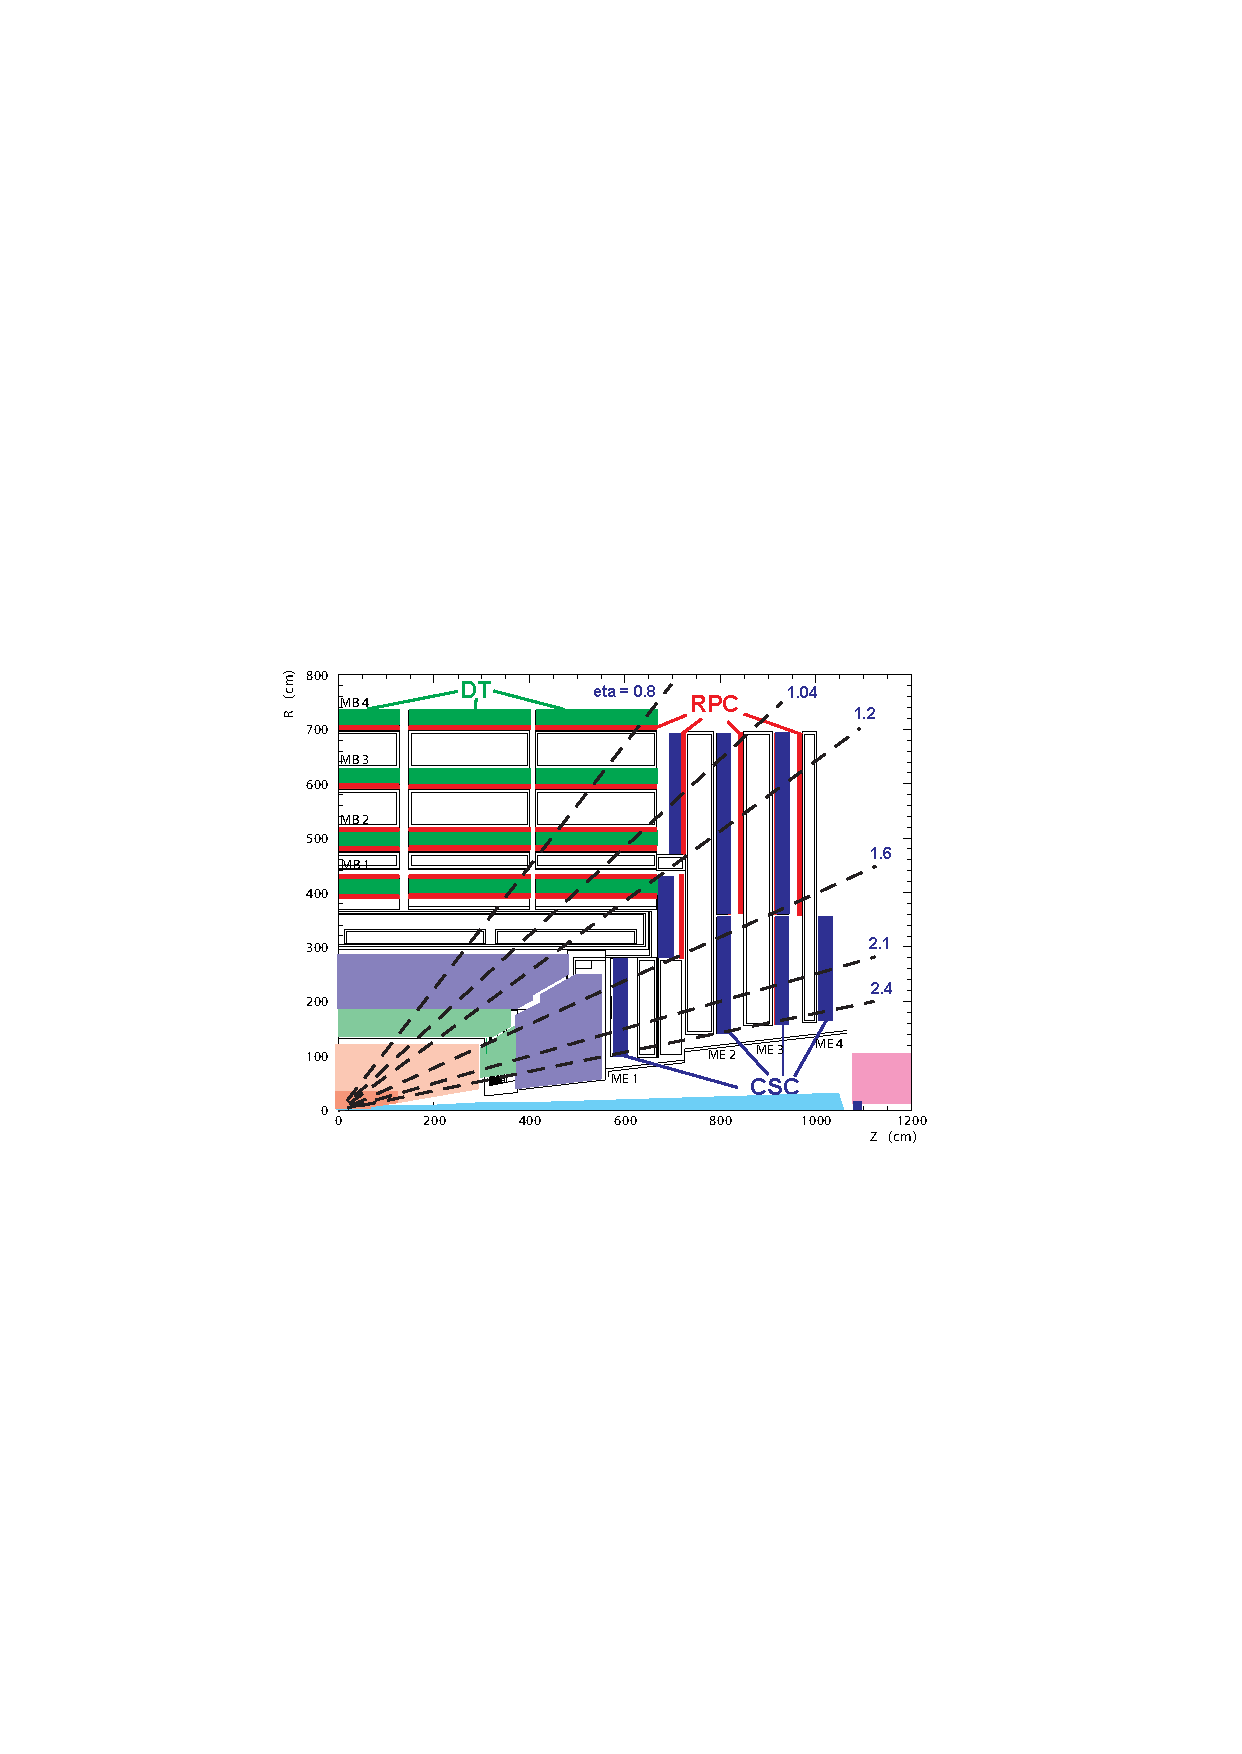
\includegraphics[width=5in]{Chapter3/importfigs/Figure_001-006.pdf}
}

\subsection{Inner Tracker}

The tracker measures the momentum of charged particles via their trajectory through a homogenous magnetic field. The tracker consists of two units, the pixel tracker and the strip tracker, both of which are made of silicon. A charged particle causes an electrical signal when passing through a silicon pixel or silicon microstrip. CMS reconstructs these electrical signals, taken at specific points of position and time, into tracks. These tracks are accurate to the 10 micrometers. The tracker is meant to have  a particle pass all the way through it, with only minimal effect particle's trajectory.

\subsubsection{Pixel Tracker}

Every silicon-pixel has a corresponding readout chip. The readout chips are soldered through the bump-bonding method. The readout chip amplifies signals from the pixel.

The pixel tracker is precise enough to distinguish the vertices of tracks originating from short-lived particles, such as bottomonia. 

\subsubsection{Strip Tracker}

\centerline{
\includegraphics[width=5in]{Chapter3/importfigs/cms_cft_09_003_fig1.png}
}

\subsection{Electromagnetic Calorimeter}

The Electromagnetic Calorimeter (ECAL) is the dedicated CMS calorimeter for detecting electrons and photons. The calorimeter is comprised of lead tungstate ($PbWO_4$) crystals arranged in cylinder about the beam, including two endcaps. The granularity of these crystals gives the ECAL excellent energy resolution, angular resolution, and spatial resolution. The ECAL is hermetic and homogenous. The data readout is fast enough that CMS can trigger off signals in the ECAL.

\centerline{
\includegraphics[width=5in]{Chapter3/importfigs/Figure_001-007.pdf}
}
 
\subsection{Hadronic Calorimeter}

The Hadronic Calorimeter (HCAL) has such a large acceptance that it can indirectly observe non-interacting particles such as neutrinos.

\centerline{
\includegraphics[width=5in]{Chapter3/importfigs/Figure_001-008.pdf}
}

\subsubsection{Hadronic Forward Calorimeters}

The Hadronic Forward Calorimeters (HF) absorbs the greatest portion of energy from collisions. As such it is designed for maximum radiative resistance.

\subsection{Muon Detector}



\subsection{Zero Degree Calorimeter}


\subsection{Particle Flow Algorithm}

\centerline{
\includegraphics[width=5.5in]{Chapter3/importfigs/Figure_001.png}
}


\subsection{Luminosity}

One of the most important quantities measured by CMS is luminosity. Luminosity is necessary to convert the number of events detected, for a given channel, into a collision cross-section. Collision cross-sections are among the primary observables predicted by theoretical physics, specifically quantum field theory.

\subsubsection{van de Meer Scanning}

\subsection{Triggering}

CMS reconstruct events faster than they can be stored on hard-drives. To account for this phenomena -- pile-up -- CMS uses a two tiered triggering system. L1 triggers are always online, and for those events that pass the L1 triggers, the High Level Triggers (HLTs) will select which events are stored as data.

\chapter{Detecting Photoproduction in Ultra-Peripheral HI Collisions}

\section{Selection on Hadronic Forward Calorimeter}

\section{Selection on Zero Degree Calorimeter}

\section{Selection on Pixel Tracker}


\chapter{Trigger Development and Performance}

\section{Introduction to Triggering}

Modern "triggering" methods began with Walther Bothe's development of the coincidence circuit. The coincidence ciruit accepts two inputs. If these inputs are recieced within the same time window, approximating coincidence, the circuit passes an output. Bothe's originally used the coincidence circuit to take data for electron-photon production in Compton scattering. Figure \ref{fig:ross} is the diagram of a coincidence circuit. 

\begin{figure}[h!]
\begin{centering}
\includegraphics[width=4in]{Chapter5/importfigs/Rossis-coincidence-circuit-appearing-in-Ref-65-The-selecting-resistance-on-the-right.png}
\par\end{centering}
\caption{Rossi circuit with three Geiger-Muller coincidence circuits. \label{fig:ross}}
\end{figure}

\section{Triggering at CMS}

At stable beams, the LHC delivers bunch crossings every 25 nanoseconds. Each bunch crossing in turn will have some 20 hadron collisions. The resulting interaction rate -- $10^9$ interactions per second -- is orders of magnitude greater than the frequency that events can be written to disk, $10^2$ events per second. CMS therefore needs a means of filtering out the most interesting $10^2$ interactions per second while declining the other $10^6$ interactions per second. 

CMS uses a two-tiered triggering system. The first tier, the L1 trigger, is hardware based. The second tier, the high-level trigger (HLT), is software based. The L1 trigger recieves raw data from the calorimeters and the muon detectors; this determines when the tracker will readout data. The raw data from the tracker, calorimeters, and muon detectors is then passed on to a computer farm running the HLT menu. The HLT then performs a simplistic reconstruction of the raw data into physics objects useful for analysis: jets, tracks, and identifiable particles. If an event passes the HLT, the raw data is permanently stored in preparation for a more complex reconstruction. 

The initial interaction rate is approximately $3.2$ $\mu s$. The L1 trigger can only pass some 1 in 1000 interactions to the HLT. The L1 trigger menu has an output rate of approximately 100 kHz. L1 achieves this rate by only considering data of reduced granularity and reduced resolution. A buffer is used to store the full event data while the L1 runs. The HLT menu reduces this to about 100 Hz as required by the limit on disk writing. 

The 2015 UPC triggers were for low multiplicity events and low transverse momentum events. Typical heavy-ion collisions are high multiplicity events. Fig.\ref{fig:eventdisplayHI} is an event display of one of the first heavy-ion collisions at CMS in 2010.

\begin{figure}[h!]
\begin{centering}
\includegraphics[width=4in]{Chapter3/importfigs/cms_firstleadcoll.jpg}
\par\end{centering}
\caption{High multiplicity PbPb collision \label{fig:eventdisplayHI}}
\end{figure}

Fig.\ref{fig:eventdisplayUPCUps} is the event display of a UPC upsilon candidate. Notice that there are only two reconstructed tracks, and that CMS is otherwise empty in all calorimeters. 

\begin{figure}[h!]
\begin{centering}
\includegraphics[width=4in]{Chapter3/importfigs/upcJpsi_run285530_lumi594_event944509077_v0.png}
\par\end{centering}
\caption{UPC Upsilon candidate \label{fig:eventdisplayUPCUps}}
\end{figure}

For this analysis, the L1 trigger applies two selections. First, the L1 checks that at least one of the HF is empty. This is the most important part of the trigger in so far as it suppressed the hadronic contamination of the dataset. Then, if there is at least 5 GeV of energy deposited in the ECAL, the event passes to the HLT. 

Low multiplicity events are difficult to distinguish from background. To compensate, the HLT in turn requires that there be at least once reconstructed track from the pixel tracker, to make sure that there are particles that will be reconstructed by the complete tracker. Only the pixel tracker is used for these HLTs to increase the speed of reconstruction while decreasing needed computer cycles. 

\section{Author's Contributions}

In preparation for the 2015 heavy-ion run and the 2016 p-Pb run, I prepared high-level trigger menus for the CMS Forward-HI group. This trigger menu was optimized for firing on ultra-peripheral collisions. I tested the menu's performance on Monte Carlo generated by STARLIGHT and reconstructed through a GEANT4 simulation of CMS. During the experiment, I was present at CERN to monitor the trigger rates and deliver daily reports on their performance. 

CMSSW includes an emulator for the L1 trigger. This software can re-emulate alternative L1 menus on previously taken CMS data. The performance of a trigger on the 2011 PbPb data, taken at $\sqrt{s_NN} = 2.7 TeV$ is extrapolated to the higher energy, $\sqrt{s_NN} = 5.2 TeV$, of the 2015 PbPb run.

I tested my HLT menu on both STARLIGHT MC and on data from the 2011 Pb+Pb run. STARLIGHT is a MC generator for ultra-peripheral collisions, in particular for the vector-meson photoproduction channels. I used STARLIGHT to generate MC sets for $Pb+Pb\rightarrow J/\Psi+Pb+Pb$ and $Pb+Pb\rightarrow \Upsilon(1s)+Pb+Pb$. I then used CMSSW to test the performance of the component bits of the HLT paths with respect to these MC sets. 

\begin{figure}[h!]
\begin{centering}
\includegraphics[width=4in]{Chapter5/importfigs/triggerRateExample.png}
\par\end{centering}
\caption{Example of trigger rate. \label{fig:trigRate}}
\end{figure}

It was my duty to carefully observe the state of the UPC triggers during the heavy-ion run. If the total HLT rate ever drifted above 100 Hz, the HLT menu could crash and CMS lose considerable data. It was important for the trigger contacts to make sure that there HLT paths were behaving stablely. I also analyzed express physics data to test that the vector-meson triggers saw appropriate mass resonances.


\section{Studies from Trigger Menus}

The UPC HLTs I designed are useful for a variety of physics studies. In particular, vector meson photoproduction, light-by-light scattering, and UPC particle correlations. 

The single and double muon UPC triggers are adequate for studies of vector-meson photoproduction. As of this writing, the Forward-HIN group has ongoing studies of UPC $J/\Psi$ and UPC $\Upsilon(1s)$ in both the 2015 PbPb and 2016 pPb data. 

\chapter{Data Analysis}

In this chapter our data sample will be analyzed according to the framework provided by Yoshikata Hatta. The angular correlation of jets is taken, and event mixing is used to factor out acceptance effects. 

\chapter{Systematic uncertainties}

\begin{figure}[h!]
\begin{centering}
\includegraphics[width=5in]{Chapter7/importfigs/pt_sys_thesis.pdf}
\par\end{centering}
\caption{Jet Pt sys. \label{fig:ptSys}}
\end{figure}

\begin{figure}[h!]
\begin{centering}
\includegraphics[width=5in]{Chapter7/importfigs/vert_sys_thesis.pdf}
\par\end{centering}
\caption{Vertex sys. \label{fig:vertSys}}
\end{figure}

\begin{figure}[h!]
\begin{centering}
\includegraphics[width=5in]{Chapter7/importfigs/rcorr_sys_thesis.pdf}
\par\end{centering}
\caption{Correction factor. \label{fig:rcorrSys}}
\end{figure}

\chapter{Results and conclusions}

In this chapter, the angular anisotropy of the elliptic gluons is compared to theoretical predictions from variations of NLO-QCD.

%\global\long\def\bibname{References}
%\nocite{*}
%\bibliographystyle{apalike2}

\bibliographystyle{Biblio/utphys}
\bibliography{Biblio/allcites}
%\appendix
%
\chapter{Monte Carlo Generation and Reconstruction}

The Monte Carlo (MC) for this analysis was generated using the RAPGAP software package. RAPGAP is a generator for eletron-proton MC. The structure functions measured at HERA are used to model a variety of diffractive processes. Each event has a characteristic energy for the virtual photon exchanged by the electron and proton. This photon energy is used to reweigh the MC to model the energy distribution of the Weizacker Williams photon flux. 

\begin{equation}
w(E) = \frac{\mathrm{d} N^{eff}_\gamma}{\mathrm{d} E} / \frac{\mathrm{d} N^{RAPGAP}_\gamma }{\mathrm{d} E}
\end{equation}
$\mathrm{d} N^{RAPGAP}_\gamma / \mathrm{d} E$ is obtained by fitting the formula for the total electron-proton cross-section, $\sigma_{\gamma p}$ to the RAPGAP MC's energy distribution. 

\begin{figure}[h!]
\begin{centering}
\includegraphics[width=4in]{Appendix1/importfigs/rapgap_diagram.png}
\par\end{centering}
\caption{RAPGAP process: boson-gluon fusion. \label{fig:rapgap_diagram}}
\end{figure}

\begin{equation}
\frac{\mathrm{d}^2 \sigma_{ep} }{\mathrm{d} y \; \mathrm{d} Q^2} = \frac{\alpha}{2 \pi Q^2}\left ( \frac{1+(1-y)^2)}{y} - \frac{2(1-y)}{y}\cdot \frac{Q^2_{min}}{Q^2} \right )\cdot \sigma^{tot}_{\gamma^*p}(W_{\gamma^*p}),
\end{equation}
where 
\begin{equation}
Q^2_{min}\approx \frac{m_e^2 \; y^2}{1-y}.
\end{equation}
In this context, $y$ is the energy fraction carried away from the electron by the mediating virtual photon, $Q^2$ is the photon virtuality, $m_e$ is the electron mass, $\sigma^{tot}_{\gamma^*p}(W_{\gamma^*p})$ is the total photon-proton cross section, and $W_{\gamma^*p}$ is the center of mass energy of the photon-proton collision. 

\begin{figure}%
    \centering
    \subfloat[label 1]{{\includegraphics[width=7.cm]{Appendix1/importfigs/before_fit.png} }}%
    \qquad
    \subfloat[label 2]{{\includegraphics[width=7.cm]{Appendix1/importfigs/after_fit.png} }}%
    \caption{Left: Energy Distribution Before Fitting, Right: Energy Distribution After Fitting}%
    \label{fig:patKennyPlots}%
\end{figure}

\end{document}